

\section{Introduction}

Disagreements about the utility of programming languages are
as old as programming itself. Today,
these ``language wars'' become increasingly heated, and less meaningful, as
more people are working with more languages on more platforms in settings of
greater variety, e.g., from mobile to datacenters.

In this paper, we contribute to the discussion by implementing a well
defined algorithm in four different languages, C++, Java, Go, and
Scala. In all implementations, we use the default, idiomatic data
structures in each language, as well as default type systems, memory
allocation schemes, and default iteration constructs. All four
implementations stay very close to the formal specification of the
algorithm and do not attempt any form of language specific
optimization or adaption.

The benchmark itself is simple and compact. Each implementation
contains some scaffold code, needed to construct test cases
allowing to benchmark the algorithm, and the implementation of the
algorithm itself.

The algorithm employs many language features, in particular,
higher-level data structures (lists, maps, lists and arrays of sets
and lists), a few algorithms (union/find, dfs / deep recursion, and
loop recognition based on Tarjan), iterations over collection types,
some object oriented features, and interesting memory allocation
patterns.  We do not explore any aspects of multi-threading, or higher
level type mechanisms, which vary greatly between the languages. We
also do not perform heavy numerical computation, as this omission
allows amplification of core characteristics of the language
implementations, specifically, memory utilization
patterns.

We believe that this approach highlights features and characteristics
of the languages and allows an almost fair comparison along the
dimensions of source code complexity, compilers and default libraries,
compile time,
binary sizes, run-times, and memory footprint. The differences along
these dimensions are surprisingly large.

After publication of the benchmark internally at Google, several
engineers produced highly optimized versions of the benchmark.  We
describe many of the performed optimizations, which were mostly
targeting run-time performance and code complexity. While this
evaluation is an anecdotal comparison only, the benchmark itself, as
well as the subsequent tuning efforts, point to typical performance
pain points in the respective languages.

The rest of this paper is organized as follows. We briefly introduce
the four languages in section \ref{contenders}.  We introduce the
algorithm and provide instructions on
how to find, build, and run it, in section \ref{algo}. 
We highlight core language properties in section
\ref{props}, as they are needed to understand the implementation and
the performance properties. We describe the benchmark and
methodology in section \ref{benchmark}, which also contains the
performance evaluation. We discuss subsequent language
specific tuning efforts in section \ref{tuning}, before we conclude.
 
 

\section{The contenders}
\label{contenders}

We describe the four languages by providing links to the  
the corresponding wikipedia entries and cite the respective first paragraphs
from wikipedia. 
Readers familiar with the languages can skip to the next section.

{\em C++} \cite{lang-cpp} is a statically typed,
free-form, multi-paradigm, compiled, general-purpose programming
language. It is regarded as a "middle-level" language, as it comprises
a combination of both high-level and low-level language features.
It was developed by Bjarne Stroustrup starting in 1979 at Bell Labs as
an enhancement to the C language and originally named C with
Classes. It was renamed C++ in 1983.


{\em Java} \cite{lang-java} is
a programming language originally developed by James Gosling at Sun
Microsystems (which is now a subsidiary of Oracle Corporation) and
released in 1995 as a core component of Sun Microsystems' Java
platform. The language derives much of its syntax from C and C++ but
has a simpler object model and fewer low-level facilities. Java
applications are typically compiled to byte-code (class file) that can
run on any Java Virtual Machine (JVM) regardless of computer
architecture. Java is a general-purpose, concurrent, class-based,
object-oriented language that is specifically designed to have as few
implementation dependencies as possible. It is intended to let
application developers "write once, run anywhere". Java is currently
one of the most popular programming languages in use, and is widely
used from application software to web applications.


{\em Go} \cite{lang-go} is a
compiled, garbage-collected, concurrent programming language developed
by Google Inc.  The initial design of Go was started in September 2007
by Robert Griesemer, Rob Pike, and Ken Thompson, building on previous
work related to the Inferno operating system. Go was officially
announced in November 2009, with implementations released for the
Linux and Mac OS X platforms. At the time of its launch, Go was not
considered to be ready for adoption in production environments. In May
2010, Rob Pike stated publicly that Go is being used "for real stuff"
at Google.

{\em Scala} \cite{lang-scala}
is a multi-paradigm programming language designed to integrate
features of object-oriented programming and functional
programming. The name Scala stands for "scalable language", signifying
that it is designed to grow with the demands of its users.

Core properties of these languages are:

\begin{itemize}

\item C++ and Go are statically compiled, both Java and Scala run on
  the JVM, which means code is compiled to Java Byte Code, which is 
  interpreted and/or compiled dynamically.

\item All languages but C++ are garbage collected, where Scala and
  Java share the same garbage collector.

\item C++ has pointers, Java and Scala has no pointers, and Go makes
  limited use of pointers.

\item C++ and Java require statements being terminated with a
  ';'. Both Scala and Go don't require that. Go's algorithm enforces
  certain line breaks, and with that a certain coding style. While Go's
  and Scala's algorithm for semicolon inference are 
  different, both algorithms are intuitive and powerful.

\item C++, Java, and Scala don't enforce specific coding styles. As a
  result, there are many of them, and many larger programs have many
  pieces written in different styles. The C++ code is written
  following Google's style guides, the Java and Scala code (are trying
  to) follow the official Java style guide. Go's programming style is
  strictly enforced -- a Go program is only valid if it comes
  unmodified out of the automatic formatter {\tt gofmt}.

\item Go and Scala have powerful type inference, making explicit type
  declarations very rare. In C++ and Java everything needs to be
  declared explicitly.

\item C++, Java, and Go, are object-oriented. Scala is object-oriented
  and functional, with fluid boundaries.

\end{itemize}


\section{The Algorithm}
\label{algo}

The benchmark is an implementation of the loop recognition algorithm
described in "Nesting of reducible and irreducible loops", by Havlak,
Rice University, 1997, \cite{havlak}.  The algorithm itself is an
extension to the algorithm described R.E. Tarjan, 1974, Testing flow
graph reducibility \cite{Tarjan:1983}. 
It further employs the Union/Find algorithm
described in "Union/Find Algorithm", Tarjan, R.E., 1983, Data
Structures and Network Algorithms \cite{Tarjan:1973}.

The algorithm formulation in Figure \ref{algofig}, as well as the
various implementations, follow the nomenclature using variable names
from the algorithm in Havlak's paper, which in turn follows the Tarjan
paper.

\begin{figure}
%\includegraphics[width=85mm]{algo2cropped.pdf}
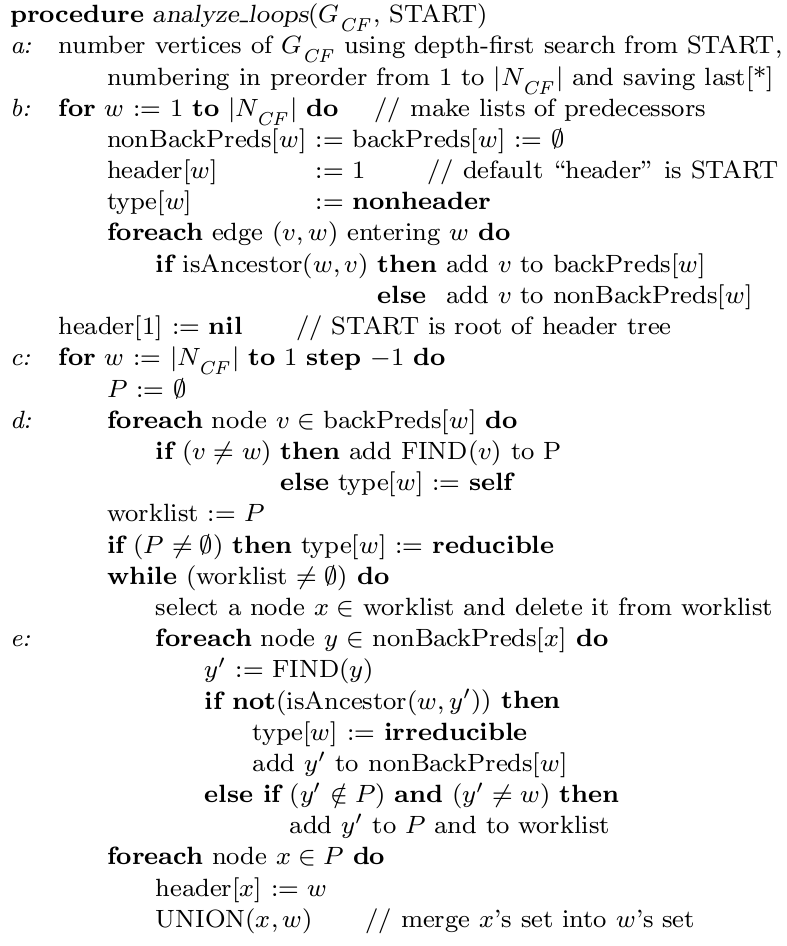
\includegraphics[width=85mm]{havlaklarge.png}
\caption{Finding headers of reducible and irreducible loops. This 
    presentation is a literal copy from the original paper \cite{havlak}}
\label{algofig}
\end{figure}

The full benchmark sources are available as open-source, hosted
by Google code at {\tt http://code.google.com/p/} in the project
{\tt multi-language-bench}.
The source files contain the main algorithm
implementation, as well as dummy classes to
construct a control flow graph (CFG), a loop structure graph (LSG),
and a driver program for benchmarking (e.g., {\tt LoopTesterApp.cc}).

As discussed, after an internal version of this document was published
at Google, several engineers created optimized versions of the
benchmark. We feel that the optimization techniques applied for each
language were interesting and indicative of the issues
performance engineers are facing in their every day experience.  The
optimized versions are kept in the {\em Pro} versions of the
benchmarks. At time of this writing, the {\tt cpp\_pro} version
depended strongly on Google specific code and could not be open-sourced.
All directories in Figure \ref{sourcedirs} are found in the
{\tt havlak} directory.

Each directory contains a {\tt Makefile} and supports three
methods of invocation:

\begin{footnotesize}
\begin{verbatim}
  make       # build benchmark
  make run   # run benchmark
  make clean # clean up build artifacts
\end{verbatim}
\end{footnotesize}

Path names to compilers and libraries can be overridden
on the command lines. Readers interested in running the benchmarks
are encouraged to study the very short {\tt Makefiles} for 
more details.

\begin{figure}
\begin{tabular}{ll}
{\tt\small src           }  & README file and auxiliary scripts  \\
{\tt\small src/cpp       }  & C++ version \\
{\tt\small src/cpp\_pro  }  & Improved by Doug Rhode \\
{\tt\small src/scala     }  & Scala version \\
{\tt\small src/scala\_pro}  & Improved by Daniel Mahler \\
{\tt\small src/go        }  & Go version \\
{\tt\small src/go\_pro   }  & Improved by Ian Taylor \\
{\tt\small src/java      }  & Java version \\
{\tt\small src/java\_pro }  & Improved by Jeremy Manson \\
{\tt\small src/python    }  & Python version (not discussed here) \\
\end{tabular}
\caption{Benchmark source organization (at the time of this writing,
the cpp\_pro version could not yet be open-sourced)}
\label{sourcedirs}
\end{figure}


\section{Implementation Notes}
\label{props}

This section highlights a few core language properties, as necessary to 
understanding the benchmark sources and performance characteristics. 
Readers familiar with the languages can safely skip to the next section.

\subsection{Data Structures}

The key data structures for the implementation of the algorithm are
shown in Figure \ref{datastructs}. Please note again that we are
strictly following the algorithm's notation. We do not seek to apply
any manual data structure optimization at this point. We use the
non object-oriented, quirky notation of the paper, and we only
use the languages' default containers.

\begin{figure}
\begin{tabular}{ll}
{\tt\small non\_back\_preds} & an array of sets of int's  \\
{\tt\small back\_preds} & an array of lists of int's  \\
{\tt\small header} & an array of int's \\
{\tt\small type  } & an array of char's  \\
{\tt\small last  } & an array of int's \\
{\tt\small nodes } & an array of union/find nodes \\
{\tt\small number} & a map from basic blocks to int's \\
\end{tabular}
\caption{Key benchmark data structures, modeled after the original paper}
\label{datastructs}
\end{figure}

\subsubsection{C++} 
With the standard library and templates, these data structures are defined the following way in C++ using stack local variables:

\begin{footnotesize}
\begin{verbatim}
  typedef std::vector<UnionFindNode>  NodeVector;
  typedef std::map<BasicBlock*, int>  BasicBlockMap;
  typedef std::list<int>              IntList;
  typedef std::set<int>               IntSet;
  typedef std::list<UnionFindNode*>   NodeList;
  typedef std::vector<IntList>        IntListVector;
  typedef std::vector<IntSet>         IntSetVector;
  typedef std::vector<int>            IntVector;
  typedef std::vector<char>           CharVector;
[...]
    IntSetVector       non_back_preds(size);
    IntListVector      back_preds(size);
    IntVector          header(size);
    CharVector         type(size);
    IntVector          last(size);
    NodeVector         nodes(size);
    BasicBlockMap      number;
\end{verbatim}
\end{footnotesize}

The size of these data structures is known at run-time and the {\tt
  std::} collections allow pre-allocations at those sizes, except for
the map type.

\subsubsection{Java} 

Java does not allow arrays of generic types. However, lists are
index-able, so this code is permissible:

\begin{footnotesize}
\begin{verbatim}
List<Set<Integer>>  nonBackPreds = 
               new ArrayList<Set<Integer>>();
List<List<Integer>> backPreds = 
               new ArrayList<List<Integer>>();
int[]               header = new int[size];
BasicBlockClass[]   type = 
               new BasicBlockClass[size];
int[]               last = new int[size];
UnionFindNode[]     nodes = new UnionFindNode[size];
Map<BasicBlock, Integer> number = 
               new HashMap<BasicBlock, Integer>();
\end{verbatim}
\end{footnotesize}

However, this appeared to incur tremendous GC overhead. In order to
alleviate this problem we slightly rewrite the code, which reduced GC
overhead modestly.

\begin{footnotesize}
\begin{verbatim}
    nonBackPreds.clear();
    backPreds.clear();
    number.clear();
    if (size > maxSize) {
      header = new int[size];
      type = new BasicBlockClass[size];
      last = new int[size];
      nodes = new UnionFindNode[size];
      maxSize = size;
    }
\end{verbatim}
\end{footnotesize}

Constructors still need to be called:

\begin{footnotesize}
\begin{verbatim}
    for (int i = 0; i < size; ++i) {
      nonBackPreds.add(new HashSet<Integer>());
      backPreds.add(new ArrayList<Integer>());
      nodes[i] = new UnionFindNode();
    }
\end{verbatim}
\end{footnotesize}

To reference an element of the {\tt ArrayLists},  the {\tt get/set}
methods are used, like this:

\begin{footnotesize}
\begin{verbatim}
   if (isAncestor(w, v, last)) {
            backPreds.get(w).add(v);
          } else {
            nonBackPreds.get(w).add(v);
          }
\end{verbatim}
\end{footnotesize}


\subsubsection{Scala}

Scala allows arrays of generics, as an array is just a language
extension, and not a built-in concept. Constructors still need to be
called:

\begin{footnotesize}
\begin{verbatim}
var nonBackPreds = new Array[Set[Int]](size)
var backPreds    = new Array[List[Int]](size)
var header       = new Array[Int](size)
var types        = 
           new Array[BasicBlockClass.Value](size)
var last         = new Array[Int](size)
var nodes        = new Array[UnionFindNode](size)
var number       = 
   scala.collection.mutable.Map[BasicBlock, Int]()

for (i <- 0 until size) {
    nonBackPreds(i) = Set[Int]()
    backPreds(i)    = List[Int]()
    nodes(i)        = new UnionFindNode()
}
\end{verbatim}
\end{footnotesize}

With clever use of parenthesis (and invocation of {\tt apply()}
accesses become more canonical, e.g.:


\begin{footnotesize}
\begin{verbatim}
     if (isAncestor(w, v, last)) {
         backPreds(w) = v :: backPreds(w)
     } else {
         nonBackPreds(w) += v
     }
\end{verbatim}
\end{footnotesize}

\subsubsection{Go}

This language offers the {\tt make} keyword in addition to the {\tt
  new} keyword.  {\tt Make} takes away the pain of the explicit
constructor calls. A map is a built-in type, and has a special syntax,
as can be seen in the 1st line below. There is no {\tt set} type, so in
order to get the same effect, one can use a map to {\tt bool}. While
maps are built-in, lists are not, and as a result accessors and
iterators become non-canonical.

\begin{footnotesize}
\begin{verbatim}
 nonBackPreds := make([]map[int]bool, size)
 backPreds := make([]list.List, size)
 number := make(map[*cfg.BasicBlock]int)
 header := make([]int, size, size)
 types := make([]int, size, size)
 last := make([]int, size, size)
 nodes := make([]*UnionFindNode, size, size)

 for i := 0; i < size; i++ {
 nodes[i] = new(UnionFindNode)
 }
\end{verbatim}
\end{footnotesize}




%------------------------------------------------------------------------------


\subsection{Enumerations}

To enumerate the various kinds of loops an
enumeration type is used. The following subsections show
what the languages offer to express compile time constants.

\subsubsection{C++}
In C++ a regular {\tt enum} type can be used

\begin{footnotesize}
\begin{verbatim}
  enum BasicBlockClass {
    BB_TOP,          // uninitialized
    BB_NONHEADER,    // a regular BB
    BB_REDUCIBLE,    // reducible loop
    BB_SELF,         // single BB loop
    BB_IRREDUCIBLE,  // irreducible loop
    BB_DEAD,         // a dead BB
    BB_LAST          // Sentinel
  };
\end{verbatim}
\end{footnotesize}

\subsubsection{Java}

Java has quite flexible support for enumeration types. Specifically,
enum members can have constructor parameters, and enums also offer
iteration via {\tt values()}. Since the requirements for this
specific benchmark are trivial, the code
looks similarly simple:

\begin{footnotesize}
\begin{verbatim}
  public enum BasicBlockClass {
    BB_TOP,          // uninitialized
    BB_NONHEADER,    // a regular BB
    BB_REDUCIBLE,    // reducible loop
    BB_SELF,         // single BB loop
    BB_IRREDUCIBLE,  // irreducible loop
    BB_DEAD,         // a dead BB
    BB_LAST          // Sentinel
  }
\end{verbatim}
\end{footnotesize}


\subsubsection{Scala}

In Scala, enumerations become a static instance of a type derived from
{\tt Enumeration}. The syntax below calls and increments {\tt Value()}
on every invocation (parameterless function calls don't need
parenthesis in Scala). Note that, in this regard, enums are not a
language feature, but an implementation of the method {\tt
  Enumeration.Value()}.  {\tt Value} also offers the ability to
specify parameter values, similar to the Java enums with constructors.

\begin{footnotesize}
\begin{verbatim}
  class BasicBlockClass extends Enumeration {
  }
  object BasicBlockClass extends Enumeration {
    val BB_TOP,      // uninitialized
    BB_NONHEADER,    // a regular BB
    BB_REDUCIBLE,    // reducible loop
    BB_SELF,         // single BB loop
    BB_IRREDUCIBLE,  // irreducible loop
    BB_DEAD,         // a dead BB
    BB_LAST = Value  // Sentinel
  }
\end{verbatim}
\end{footnotesize}

\subsubsection{Go}

Go has the concept of an {\tt iota} and initialization expression. For
every member of an enumeration (constants defined within a {\tt const}
block), the right hand side expression will be executed in full, with
{\tt iota} being incremented on every invocation. {\tt iota} is being reset on
encountering the {\tt const} keyword. This makes for flexible initialization
sequences, which are not shown, as the use case is trivial. Note that
because of Go's powerful line-breaking, not even a comma is needed. Furthermore,
because of Go's symbol exporting rules, the first characters of the
constants are held lower case (see comments on symbol binding later).

\begin{footnotesize}
\begin{verbatim}
const (
 _             = iota // Go has the iota concept
 bbTop                // uninitialized
 bbNonHeader          // a regular BB
 bbReducible          // reducible loop
 bbSelf               // single BB loop
 bbIrreducible        // irreducible loop
 bbDead               // a dead BB
 bbLast               // sentinel
)
\end{verbatim}
\end{footnotesize}



%------------------------------------------------------------------------

\subsection{Iterating over Data Structures}

\subsubsection{C++}

C++ has no "special" built-in syntactical support for iterating over
collections (e.g., the upcoming range-based for-loops in
C++0x). However, it does offer templates, and all basic data
structures are now available in the standard library. Since the
language support is minimal, to iterate, e.g., over a list of
non-backedges, one has to write:

\begin{footnotesize}
\begin{verbatim}
// Step d:
IntList::iterator back_pred_iter = 
           back_preds[w].begin();
IntList::iterator back_pred_end  = 
           back_preds[w].end();
for (; back_pred_iter != back_pred_end; 
       back_pred_iter++) {
     int v = *back_pred_iter;
\end{verbatim}
\end{footnotesize}

To iterate over all members of a map:

\begin{footnotesize}
\begin{verbatim}
for (MaoCFG::NodeMap::iterator bb_iter =
     CFG_->GetBasicBlocks()->begin();
    bb_iter != CFG_->GetBasicBlocks()->end(); 
      ++bb_iter) {
    number[(*bb_iter).second] = kUnvisited;
}
\end{verbatim}
\end{footnotesize}

\subsubsection{Java}

Java is aware of the base interfaces supported by collection types and
 offers an elegant language extension for easier iteration. In a
 sense, there is "secret" handshake between the run time libraries and
 the Java compiler. The same snippets from above look like the following in
 Java:

\begin{footnotesize}
\begin{verbatim}
      // Step d:
      for (int v : backPreds.get(w)) {
\end{verbatim}
\end{footnotesize}

and for the map:

\begin{footnotesize}
\begin{verbatim}
    for (BasicBlock bbIter : 
           cfg.getBasicBlocks().values()) {
      number.put(bbIter, UNVISITED);
\end{verbatim}
\end{footnotesize}

\subsubsection{Scala}

Scala offers similar convenience for iterating over lists:

\begin{footnotesize}
\begin{verbatim}
    // Step d:
    for (v <- backPreds(w)) {
\end{verbatim}
\end{footnotesize}

and for maps iterations:

\begin{footnotesize}
\begin{verbatim}
    for ((key, value) <- cfg.basicBlockMap) {
      number(value) = UNVISITED
    }
\end{verbatim}
\end{footnotesize}

These "for-comprehensions" are very powerful. Under the hood, the
compiler front-end builds closures and transforms the code into
combinations of calls to {\tt map(), flatmap{}, filter()}, and {\tt
  foreach()}. Loop nests and conditions can be expressed
elegantly. Each type implementing the base interfaces can be used in
for-comprehensions. This can be used for elegant language
extensions. On the downside - since closures are being built, there is
performance overhead. The compiler transforms the for-comprehensions
and therefore there is also has a "secret" hand-shake between
libraries and compiler. More details on Scala for-comprehensions can
be found in Section 6.19 of the Scala Language Specification
\cite{Scala-ref}.

Note that in the example, the tuple on the left side of the
arrow is not a built-in language
construct, but cleverly written code to mimic and implement tuples.

\subsubsection{Go}

Lists are not built-in, and they are also not type-safe. As a result,
iterations are more traditional and require explicit casting. For
example:

\begin{footnotesize}
\begin{verbatim}
// Step d:
for ll := backPreds[w].Front(); ll != nil; 
    ll = ll.Next() {
       v := ll.Value.(int)
\end{verbatim}
\end{footnotesize}

Since maps are built-in, there is special range keyword and the language allows returning tuples:

\begin{footnotesize}
\begin{verbatim}
for i, bb := range cfgraph.BasicBlocks() {
       number[bb] = unvisited
\end{verbatim}
\end{footnotesize}

Note that lists are inefficient in Go (see performance and memory
footprint below). The GO Pro version replaces most lists with array
slices, yielding significant performance gains (~25\%),
faster compile times, and more
elegant code.  We denote removed lines with {\tt -} and the replacement
lines with {\tt +}, similarly to the output of modern {\tt diff} tools.
For example, the LSG data structure changes:

\begin{footnotesize}
\begin{verbatim}
type LSG struct {
 	root  *SimpleLoop
-       loops list.List
+       loops []*SimpleLoop
 }
\end{verbatim}
\end{footnotesize}

and references in {\tt FindLoops()} change accordingly:

\begin{footnotesize}
\begin{verbatim}
  - backPreds := make([]list.List, size)
  + backPreds := make([][]int, size)
\end{verbatim}
\end{footnotesize}

and

\begin{footnotesize}
\begin{verbatim}
- for ll := nodeW.InEdges().Front(); ll != nil; 
-     ll = ll.Next() {
-       nodeV := ll.Value.(*cfg.BasicBlock)

+ for _, nodeV := range nodeW.InEdges {
\end{verbatim}
\end{footnotesize}

Note that both Go and Scala use {\tt \_} as a placeholder.

\subsection{Type Inference}

C++ and Java require explicit type declarations.
Both Go and Scala have powerful type inference, which means that types
rarely need to be declared explicitly.

\subsubsection{Scala}

Because of Scala functional bias, variables or values must be declared
as such. However, types are inferred. For example:

\begin{footnotesize}
\begin{verbatim}
    var lastid = current
\end{verbatim}
\end{footnotesize}

\subsubsection{Go}

To declare and define a variable lastid and assign it the value from
an existing variable current, Go has a special assignment operator :=

\begin{footnotesize}
\begin{verbatim}
        lastid := current
\end{verbatim}
\end{footnotesize}

\subsection{Symbol Binding}

The languages offer different mechanism to control symbol bindings:

\subsubsection{C++}

C++ relies on the {\tt static} and {\tt external} keywords to specify symbol
bindings.

\subsubsection{Java}

Java uses packages and the {\tt public}
 keyword to control symbol binding.

\subsubsection{Scala}

Scala uses similar mechanism as Java, but there are differences in the
package name specification, which make things a bit more concise and
convenient. Details are online at \cite{scala-package-1} 
and \cite{scala-package-2}.

\subsubsection{Go}
Go uses a simple trick to control symbol binding. If a symbol's first
character is uppercase - it's being exported. 


\subsection{Member Functions}

\subsubsection{C++}

Google's coding style guidelines require that class members be
accessed through accessor functions. For C++, simple accessor
functions come with no performance penalty, as they are
inlined. Constructors are explicitly defined. For example, for
the {\tt BasicBlockEdge} class in the benchmarks, the code looks like the
following:

\begin{footnotesize}
\begin{verbatim}
class BasicBlockEdge {
 public:
  inline BasicBlockEdge(MaoCFG *cfg, 
                        int     from, 
                        int to);

  BasicBlock *GetSrc() { return from_; }
  BasicBlock *GetDst() { return to_; }

 private:
  BasicBlock *from_, *to_;
};
[...]
inline
BasicBlockEdge::BasicBlockEdge(MaoCFG  *cfg,
                               int      from_name,
                               int      to_name) {
  from_ = cfg->CreateNode(from_name);
  to_ = cfg->CreateNode(to_name);

  from_->AddOutEdge(to_);
  to_->AddInEdge(from_);

  cfg->AddEdge(this);
}
\end{verbatim}
\end{footnotesize}


\subsubsection{Java}

Java follows the same ideas, and the resulting code looks similar:

\begin{footnotesize}
\begin{verbatim}
public class BasicBlockEdge {
  public BasicBlockEdge(CFG cfg, 
                        int fromName, 
                        int toName) {
    from = cfg.createNode(fromName);
    to   = cfg.createNode(toName);

    from.addOutEdge(to);
    to.addInEdge(from);

    cfg.addEdge(this);
  }

  public  BasicBlock getSrc() { return from; }
  public  BasicBlock getDst() { return to; }

  private BasicBlock from, to;
};
\end{verbatim}
\end{footnotesize}

\subsubsection{Scala}

The same code can be expressed in a very compact fashion in Scala. The
class declaration allows parameters, which become instance variables
for every object. Constructor code can be placed directly into the
class definition. The variables {\tt from} and {\tt to} become accessible for users of
this class via automatically generated getter functions. Since
parameterless functions don't require parenthesis, such accessor
functions can always be rewritten later, and no software engineering
discipline is lost. Scala also produces setter functions,
which are named like the variables with an appended underscore. E.g.,
this code can use {\tt from\_(int)} and {\tt to\_(int)}
 without having to declare
them. The last computed value is the return value of a function,
saving on return statements (not applicable in this example)

\begin{footnotesize}
\begin{verbatim}
class BasicBlockEdge(cfg      : CFG, 
                     fromName : Int, 
                     toName   : Int) {
  var from : BasicBlock = cfg.createNode(fromName)
  var to   : BasicBlock = cfg.createNode(toName)
  
  from.addOutEdge(to)
  to.addInEdge(from)

  cfg.addEdge(this)
}
\end{verbatim}
\end{footnotesize}

\subsubsection{Go}

Go handles types in a different way. It allows declaration of types
and then the definition of member functions as traits to types. The
resulting code would look like this:

\begin{footnotesize}
\begin{verbatim}
 type BasicBlockEdge struct {
        to   *BasicBlock
        from *BasicBlock
 }

 func (edge *BasicBlockEdge) Dst() *BasicBlock {
        return edge.to
 }

 func (edge *BasicBlockEdge) Src() *BasicBlock {
         return edge.from
 }

 func NewBasicBlockEdge(cfg *CFG, from int, to int)
          *BasicBlockEdge {
       self := new(BasicBlockEdge)
       self.to = cfg.CreateNode(to)
       self.from = cfg.CreateNode(from)

       self.from.AddOutEdge(self.to)
       self.to.AddInEdge(self.from)

       return self
 }
\end{verbatim}
\end{footnotesize}

However, the 6g compiler does not inline functions and the resulting
code would perform quite poorly. Go also has the convention of
accessing members directly, without getter/setter
functions. Therefore, in the Go Pro version, the code is becoming a
lot more compact:

\begin{footnotesize}
\begin{verbatim}
 type BasicBlockEdge struct {
        Dst *BasicBlock
        Src *BasicBlock
 }
 
 func NewBasicBlockEdge(cfg *CFG, from int, to int) 
           *BasicBlockEdge {
        self := new(BasicBlockEdge)
        self.Dst = cfg.CreateNode(to)
        self.Src = cfg.CreateNode(from)

        self.Src.AddOutEdge(self.Dst)
        self.Dst.AddInEdge(self.Src)
 
        return self
 }
\end{verbatim}
\end{footnotesize}
